\section{The Tile Simulation Framework}

The previous chapter introduced the digital backend as well as discussed different design choices, namely tile size, routing configurations, and the effects of Aggregator position.
Here we describe how we simulate events of interested for these different tile configurations.

A successful design is able to record and send loss-less data for all events of interest.
In a DUNE-FD LArTPC these sources range in intensity from sub-MeV-scale radiogenic backgrounds native to the LAr to 10's of GeV scale of beam neutrinos or atmospheric neutrinos.
we consider the back-end design to be successful if and only if it provides the ability to fully capture and tramsit of all RTDs from these sources.

\subsection{The Tile Representation}

We model a tile (a group of digital nodes, or ASICs) based on the description given in Chapter~\ref{chap:qdb}.
A tile is then represented in software (Python 3) as a linked list of nodes which store pointers to the adjacent nodes or neighbors.

Every node in the tile holds two FIFO objects which store local and remote data. 
The local and remote FIFOs keep track of the total number of resets or transactions, respectively.
If a node receivs a new reset the local FIFO is written to, and the local FIFO transaction counter increases.
Similarly, the remote FIFO's transaction count is increased anytime the a write occurs on this FIFO, which happens everytime a digital node receives a packet from a neighbor node, including the aggregator node.

In the current implementation all packets sent between neighbor nodes are initially recorded on the remote FIFO.
At the beginning of a clock cycle, or a simulation step, each node first checks to see if its received an interrogation request.
If the node has received a soft interrogation request, and has data in its local FIFO, it will first send its data in the local FIFO, followed by the event-end packet.
If the node receives a hard interrogation request, the node will send local data, if any, and will send an event-end packet regardless of whether or not the local FIFO had any data.
If the node's local FIFO is emtpy, and it has not received an interrogation, it will check the empty status of the remote FIFO.
If the remote FIFO is not empty, this packet will be read and transmitted to its neighbors accordingly.

%% example local vs remote of snake
\begin{figure}
\centering
\begin{subfigure}{.5\textwidth}
  \centering
  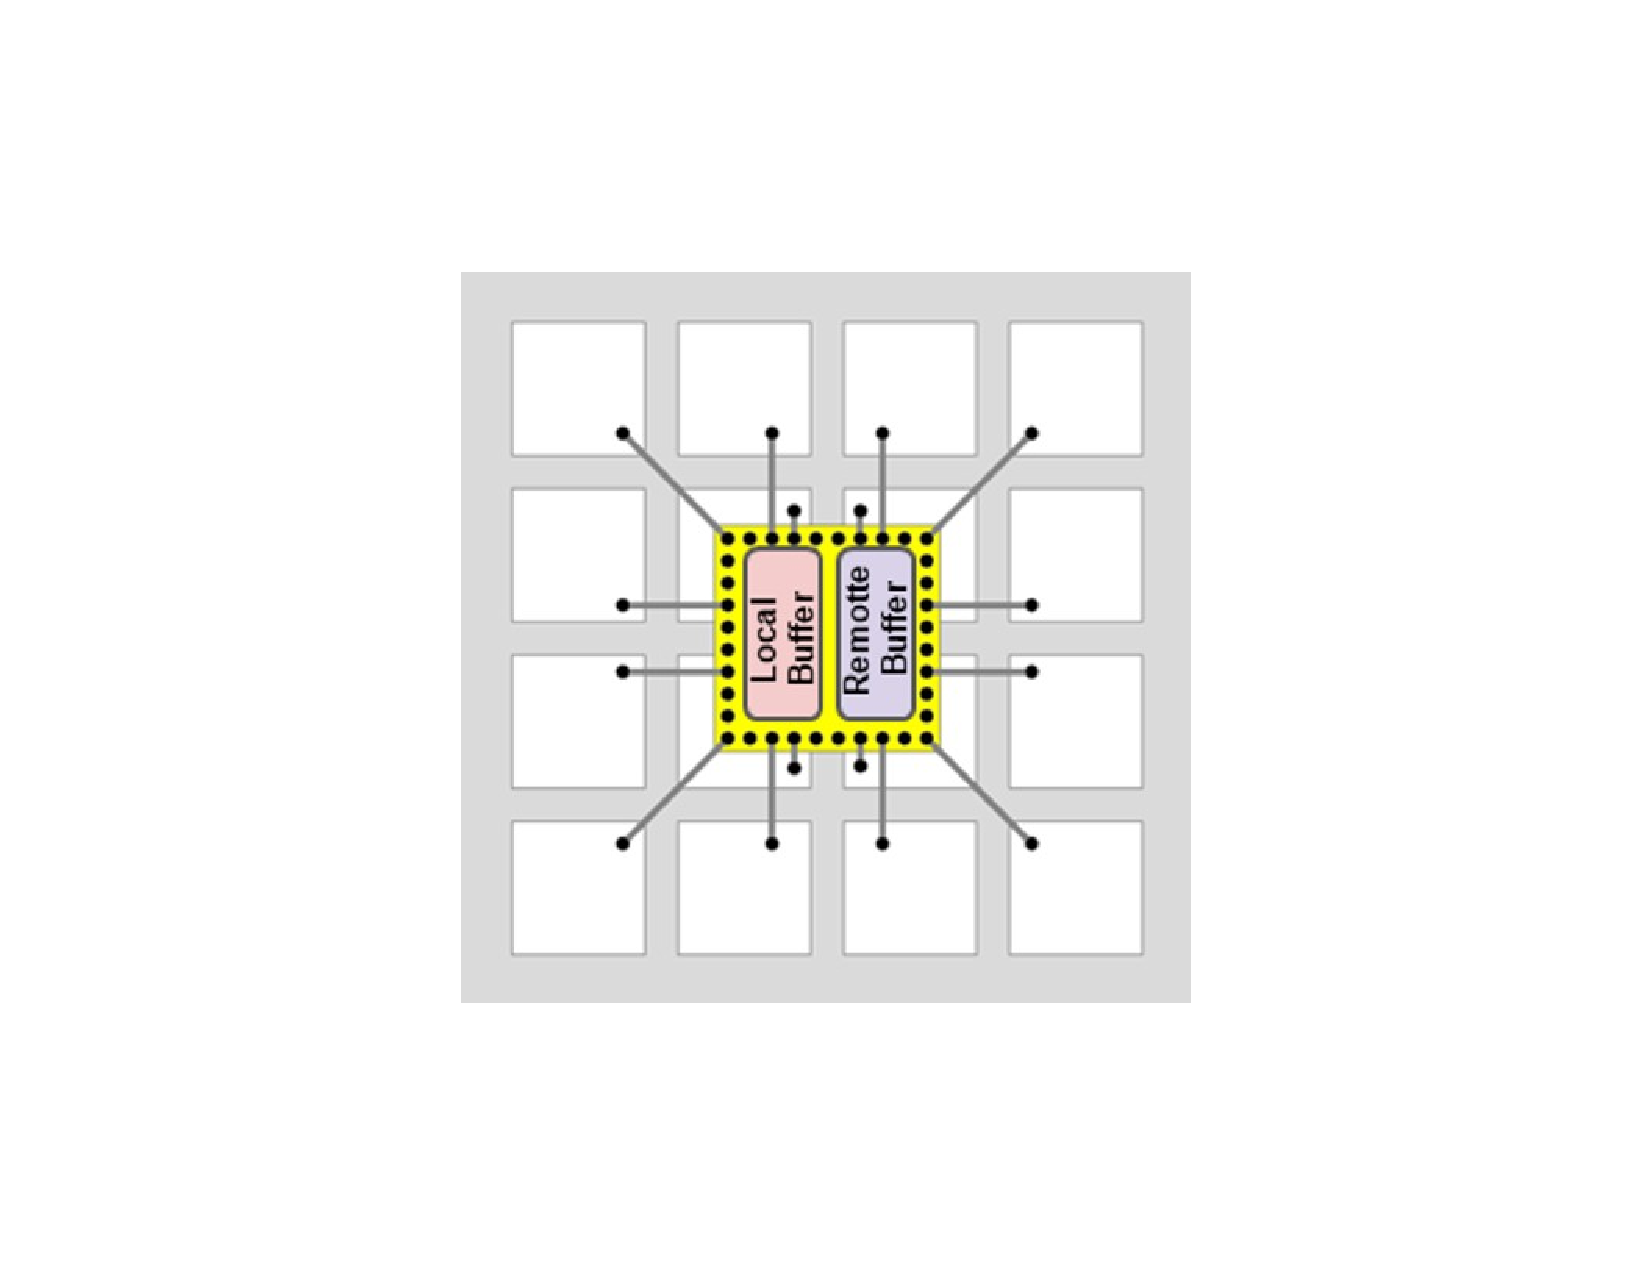
\includegraphics[width=\textwidth]{images/asic_FIFO_image.pdf}
  \caption{Individual node object stores a local FIFO and a remote FIFO object.}
\end{subfigure}%
\begin{subfigure}{.5\textwidth}
  \centering
  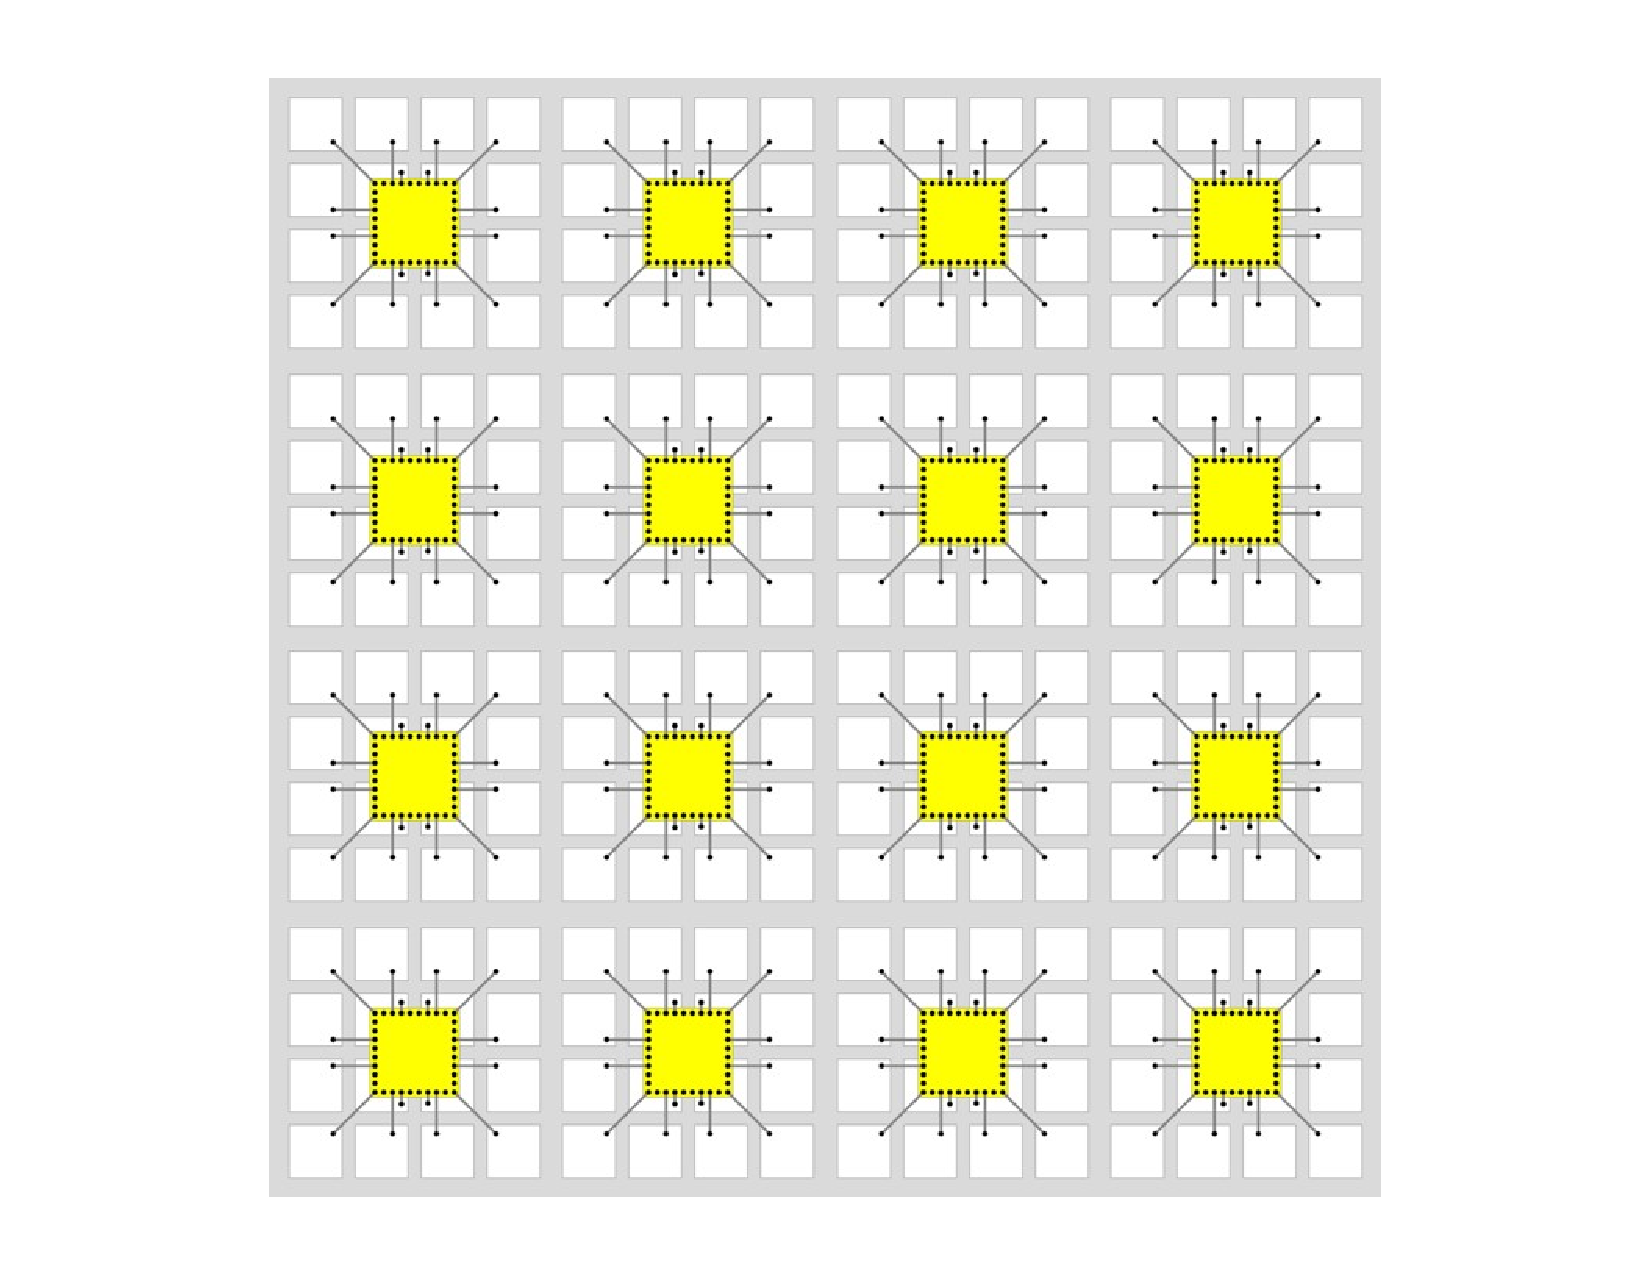
\includegraphics[width=\textwidth]{images/asic_tile_FIFO_image.pdf}
  \caption{Tile of node objects, each which have a local and remote FIFO.}
\end{subfigure}
\caption{Composition of  4$\times$4 tile.:W}
\label{fig:node_fifo_objects}
\end{figure}

There are two types of remote data to send: broadcasts and responses.
A broadcast is a register request sent to a digital node, which can only be created and sent from the aggregator node.
The responses include all other kinds of packets sent from neighbor nodes which include: data packets, event-end packets, and register response packets.

The communication packet object is a custom struct object which uses an enumerated type to differentiate the kinds of packets that the digital node can read from its remote FIFO.
Each simulated node's behavior to these incoming packets is mirrored to the digital FSM, shown in Fig.~\ref{fig:digital_fsm}.
When a node reads the packet from the remote FIFO, and uses the enumerated type to determine how to communicate the packet to its neighbors, just as is done in the firmware.

Also tested in these simulations are tiles which are have a "push" architecture.
This architecture changes the condition for a node to leave its idle state and send local data to any time that its local FIFO is not empty.
For this reason the push architecture is also more time consuming to simulate since each node can send a packet at any time, provided that it will inject a hit into its local FIFO following the procedure described in the next section.
Nodes which require an interrogation in order to send local data we refer to as the "pull" architecture.

\subsection{Injected Resets}~\label{sec:hits}

In order to speed up the executation of the python simulation reset events are precalculated and loaded into separate lists for each node.
At the beginning of every simulation time step a node checks its injected resets list against the current time.
If the current time is larger than any of the timestamps in its resets list, the resets are then removed from this list and are written to the node's local FIFO.

Resets from simulated data whether radiogenic or neutrino data can occur at any pixel and at any time.
The digital node (and the ASIC) is capable of recording multiple resets from multiple channels at the same time.
This means that it is possible for multiple different pixel resets to only contribute to on local FIFO write.
Therefore, extra care must taken when adding injected resets with channel information.

In this simulation we consider the best case timestamp measurement for each reset, which is that each digital node can record a unique reset for each channel on every new clock cycle. 
Then, procedure for combining resets from multiple channels calculates the clock cycle (timestamp) for which this node would record a timestamp for a particlar channel.
If a reset has already been recorded for this channel, the uninjected timestamp is incremented by one clock period for this node.
The above procedure then repeats until all channels have had all of their resets recorded on unique timestamps for the digital node, where only different channels can be recorded on the same timestamp.

\subsection{The Simulation Procedure}~\label{sec:process}

Upcomming sections will discuss values derived from simulating the readout of the tile. 
Here we briefly describe the simulation procedure and how the results are obtained.

The simulation loop iteratively processes a single transaction from a queue of transactions and then processes all nodes in the tile at incremental timestamps.
The timesteps used in the simulation results used here are steps 1$\unit{\mu s}$.
It is not necessary to perform smaller time steps than this, as packet transactions themselves are on the order of $\approx 50 \unit{\mu s}$, based on the endeavor protocol.
If any processed nodes generate new transactions those transactions are added to the transaction queue.

A transaction represents a 64-bit packet that is transfered between two nodes.
The sending node is reponsible for calculating the true time when this transaction would complete.
The receiving node records this byte onto its remote FIFO and performs the state check based on this packet according to Fig~\ref{fig:digital_fsm}.
Then the receiving node updates its time to its soonest clock cycle after this transaction completed.
Next, each node in the entire tile is processed one forward timestep.
If nodes are in the push state and receive a hit within this timestep window, they create a new outgoing packet, and add this packet to the transaction queue.
We note that it is only possible for processed nodes which did not receive the transaction packet to create a new packet if they are in a push-based architecture. 

The simulation is complete when all nodes have been processed up to the final requested time and no transactions are left in the queue. 
In the results presented here we process the tile for one second longer than any injected resets to ensure that the tile is fully read out.

\section{The Tile Parameters}

One goal of the simulations presented here is to parameterize different design choices in constructing both the digital nodes and the tiles.
The different parameters which we test are described in Table~\ref{table:tile_params}.

There are a total of four parameters to test: frequency stability, tile size, routing, and architecture.
Of the four parameters, we note that the frequency stability is the one unadjustable parameter.
Therefore, special care must be taken into account when designing the local oscillator for the digital nodes.

It is intuitive (and the results indicate) that improved frequency stability leads to a more stable design.
Nevertheless, we find it enlightening to demonstrate how remote buffer depths are affected in the case of a 5\% (0.5\%) clock deviation.
When a tile is created with 5\% (0.5\%) frequency deviation each node within the tile is created by randomly sampling from a gaussian distribution with a mean of 30$\unit{MHz}$ and a standard deviation of 5\% (0.5\%).
Since many ($\approx 10^4$) events are performed per tile configuration each tile is created with a random seed to ensure that each node is created with the same frequency for each test.

\begin{table}
\begin{center}
\begin{tabular}{|| p{30mm} | p{30mm} | p{90mm} ||}
 \hline
 Name & Values & Relation \\ [0.5ex]
 \hline\hline
  Frequency Standard Deviation & 0.5\%, 5\% & Packet buildup within the tile \\
 \hline
  Tile Size & 4x4, 8x8, 10x14, 16x16 & Affects total number of resets which must be routed to aggregator.\\
 \hline
  Routing & Snake, Left, and Trunk & Different trees affect packet buildup as well as transaction count  \\
 \hline
  Architecture & Push, Pull & Describes conditions for when node enters transmit-local state.~\ref{sec:local_data_packet}  \\
 \hline
\end{tabular}
\caption{The different tile parameters that are used for the effective tile search.
  The frequency drift relates the relative distribution of the frequency of adjacent oscillators.
  The tile size determines how many digital nodes are within a single tile.
  The routing configurations are described in detail in the previous chapter, and refer to how local data words are sent to the aggregator.
  The two different architectures define how the node enters the transmit local state.
  The push architecture enters whenever a new reset is acquired, whereas the pull architecture enters only when a data request is received from the aggregator.}
\end{center}
\end{table}
~\label{table:tile_params}

The other design parameters are readily configurable in either hardware (tile size) or through register configurations of the digital node (routing and, possibly, architecture).
Tile size is mostly an engineering and cost constraint.
Larger tile sizes mean the full design would require less aggregator nodes and require less tiles to parameterize.
We show results for varying tile sizes to indicate that increasing tile size may not necessarily linearly reduce cost, as larger tile sizes complicates the requirements on the digital nodes.
For this reason, the largest tile size we tested was 16 $\times$ 16.

The routing and architecture parameters help guide the digital design efforts design of the digital ASIC.
In practice it is all but certain that implemented routing for a digital tile will take on a some combination of the routing styles described here.
The reason for this is simply that is likely that some digital nodes will fail (for whatever reason) in the life time of a DUNE-FD 10 kT module.
Therefore, for the future tiles that contain hybrid routing we suggest to those users to individually analyze the sub tiles with appropriating routing and frequency distribution.

\subsection{Oscillator Drift}

Local oscillator drift was not included as a testing parameter since both the simulations and transactions occur over small time scales compared to any meaningful oscillator drift in a LArTPC.
If these drifts occur on time scales much longer than the interrogation time than the oscillator, the frequency could be continually re-calculated with the method shown in the previous chapter.
If these drifts are perodic about a mean frequency and on time scales much smaller than the interrogation time window then the drifts would average out.
In the event that clock drift timescales are on the interrogation timescale ($\approx 1\unit{s}$), then this is equivalent to a frequency uncertainty for the entire transaction cycle.
This would mean that an oscillator has a $\approx 5\%$ uncertainty in its frequnecy on each interrogation.
Such a node would not be able to reconstruct timestamps, and therefore not be able to reconstruct the z-position of charge with the required 1$\unit{ppm}$ estimated uncertainty for Q-Pix clocks~\citep{qpix:nygren:mei}.

\section{Simulating The Tile Readout}~\label{sec:simulating_tile}

The tile simulation is performed by injecting hits of some known sources which is a combination of radiogenic backgrounds and beam neutrinos.


\subsection{The Pull Architecture}

%% example local hits
\begin{figure}[]
\centering
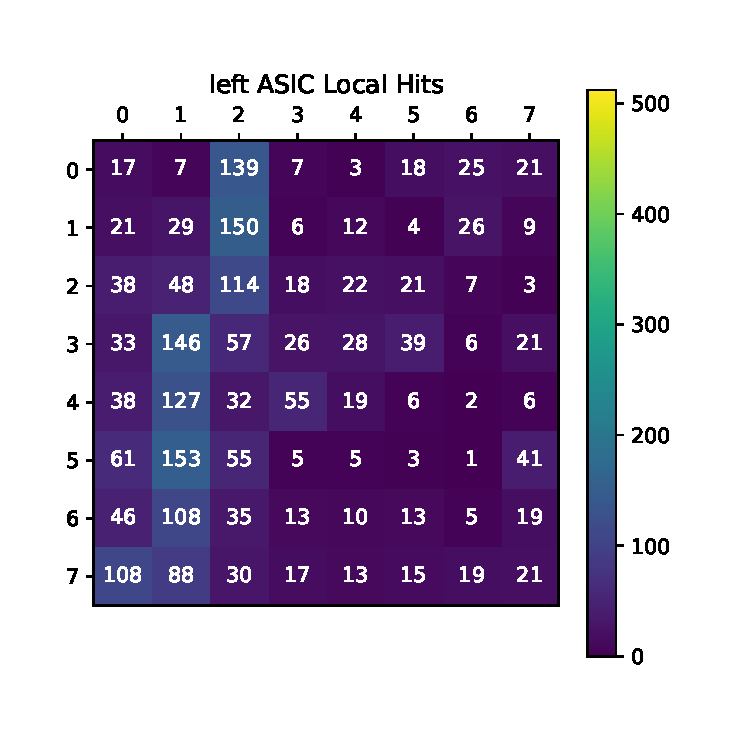
\includegraphics[width=0.5\textwidth]{images/left_asic_local.pdf}
\caption{Example local FIFO distribution of a $\approx 3\unit{GeV} \nu_{e}$ event.}
\end{figure}~\label{fig:local_buffer_hit_example}


\subsubsection{Example Neutrino Event}

%% example local vs remote of snake
\begin{figure}
\centering
\begin{subfigure}{.5\textwidth}
  \centering
  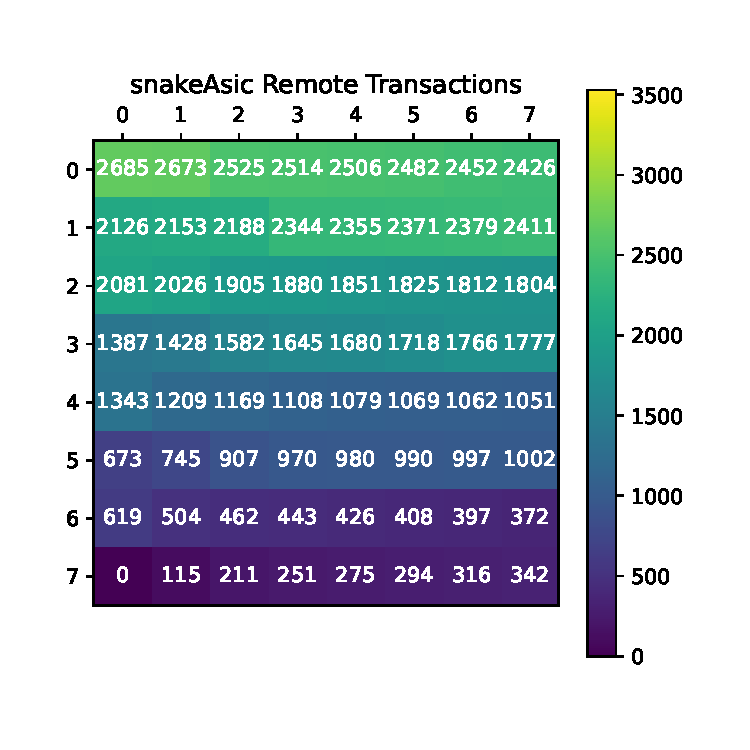
\includegraphics[width=\textwidth]{images/snake_asic_trans.pdf}
  \caption{Local FIFO Depths}
\end{subfigure}%
\begin{subfigure}{.5\textwidth}
  \centering
  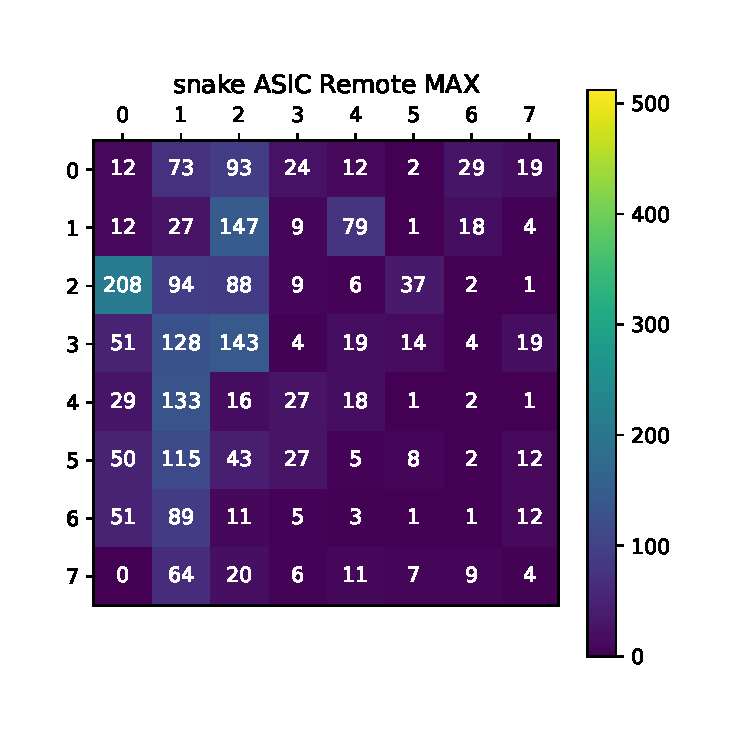
\includegraphics[width=\textwidth]{images/snake_asic_remote.pdf}
  \caption{Remote FIFO Depths}
\end{subfigure}
\caption{Example of local (a) and Remote (b) fifo depths of the example neutrino event after processing.}
\label{fig:snake_example_neutrino}
\end{figure}

%% example snake route
\begin{figure}[]
\centering
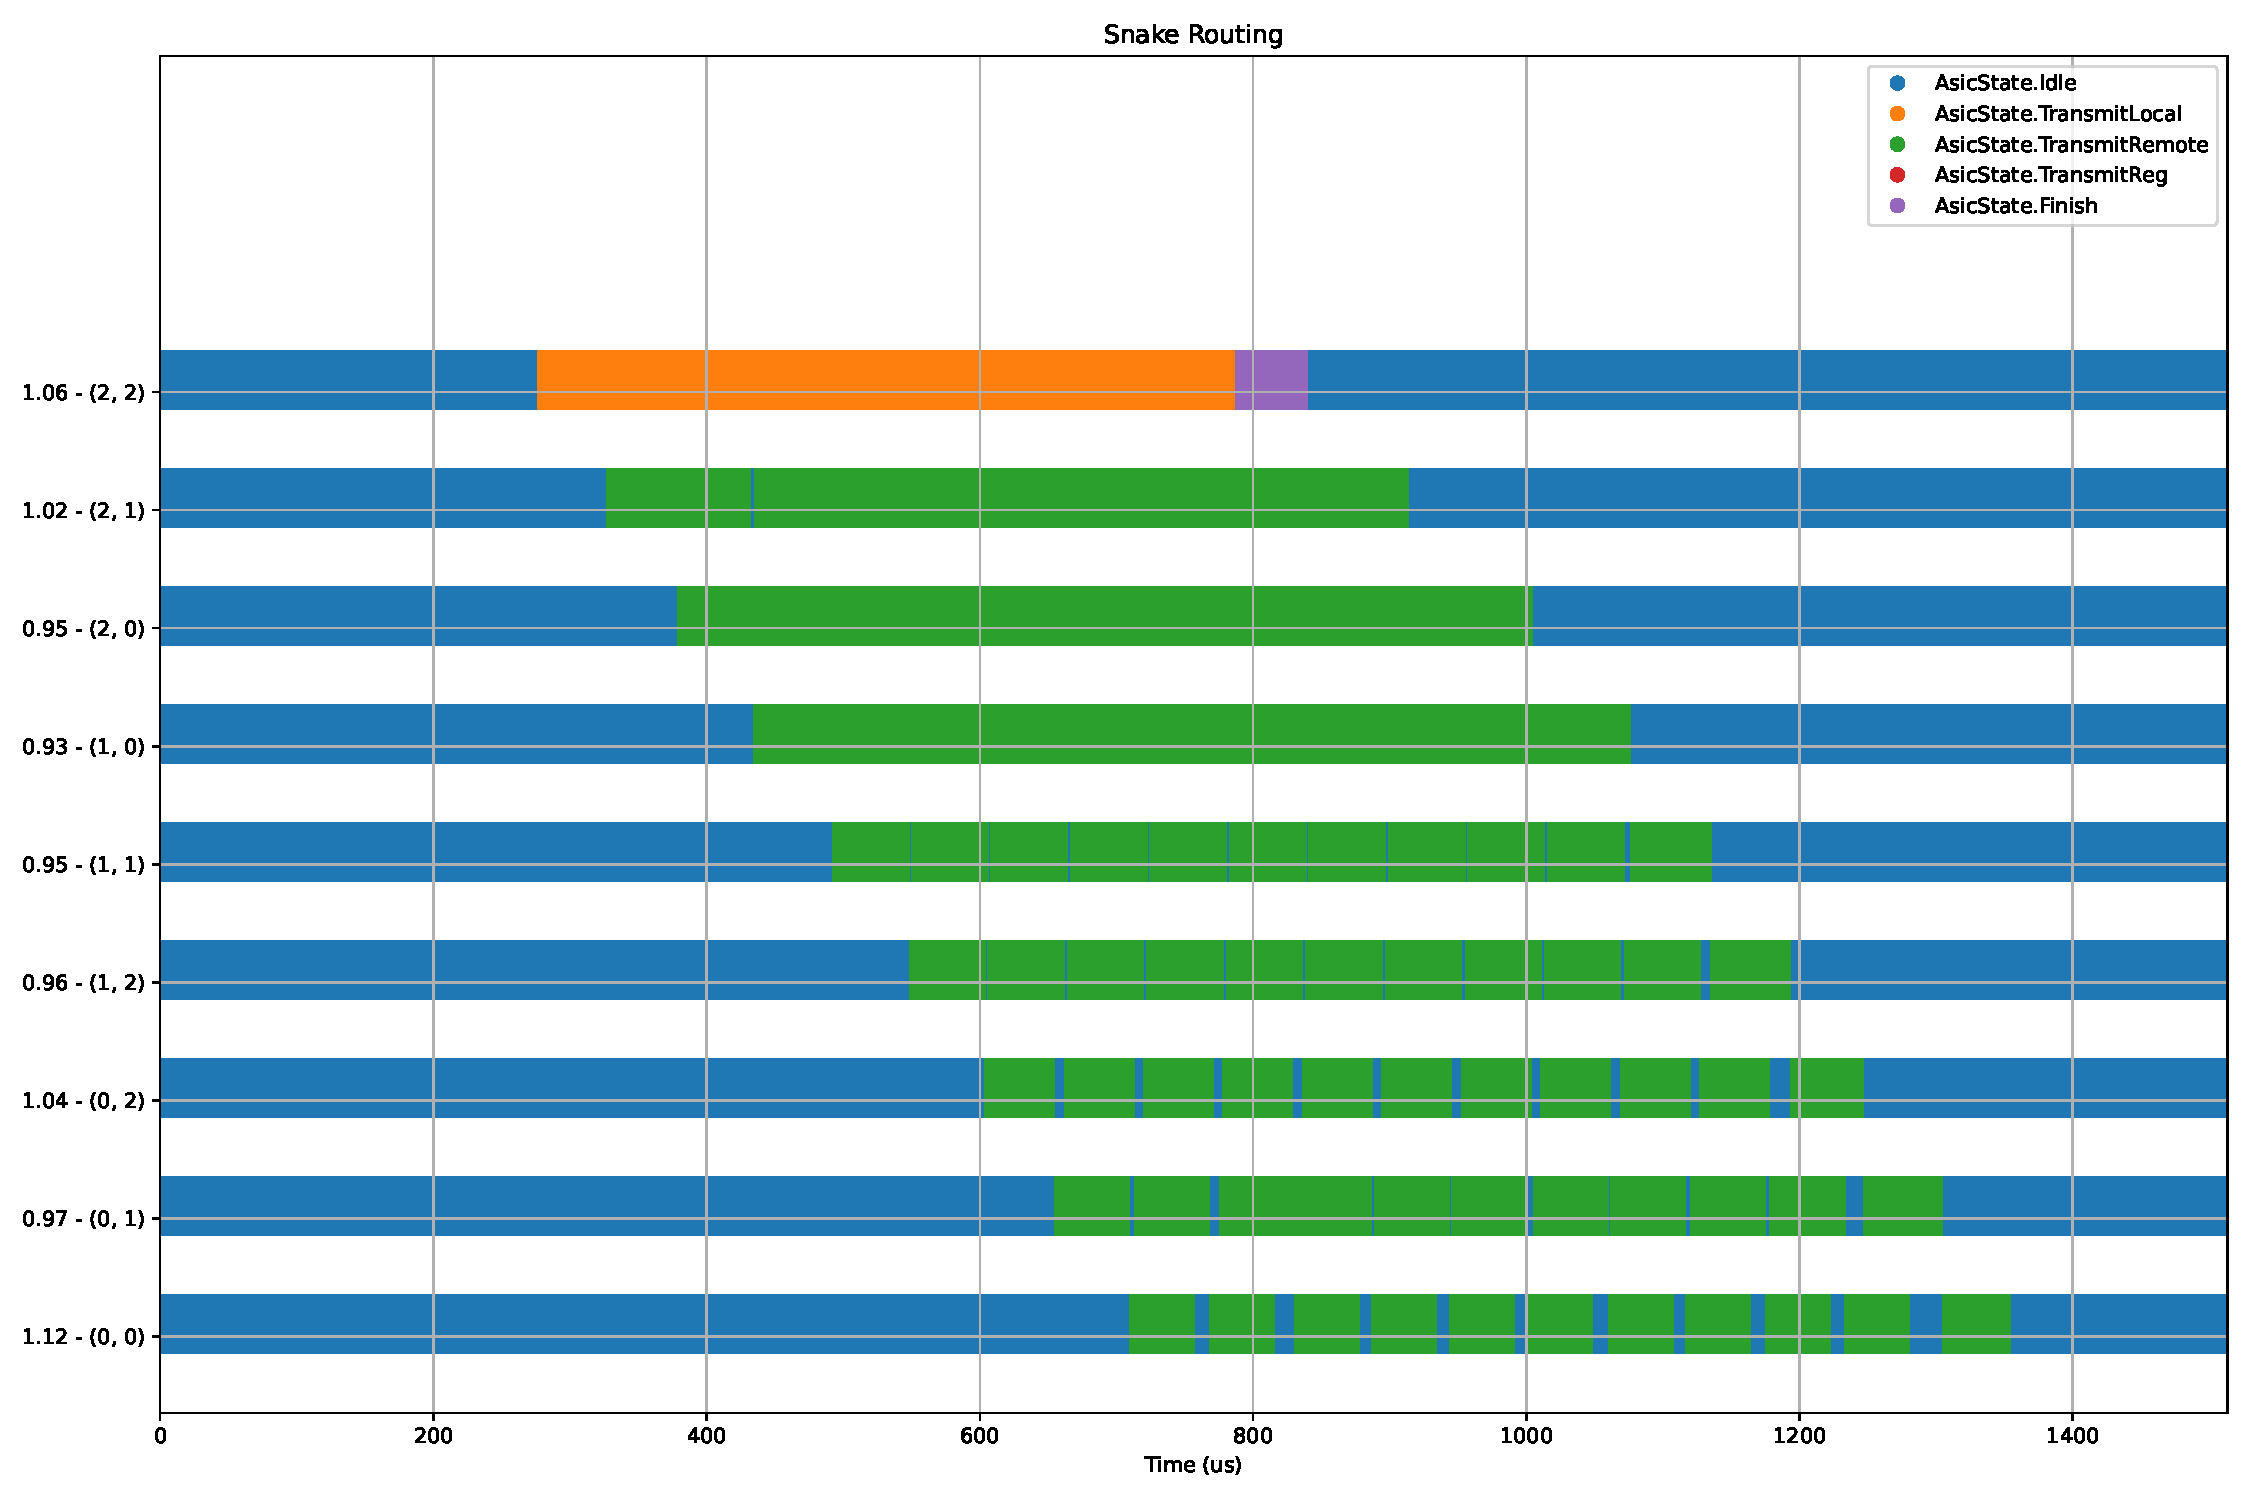
\includegraphics[width=\textwidth]{images/snake_timer.pdf}
\caption{Example of packet drift in the simulation framework.
  Packets drift apart in time as they are sent from slower to faster ASICs.
  Therefore, there is a possiblity of packet drift and asynchronous packet sending which depends on the magnitude of the frequency drift between neighbor ASICs.}
\end{figure}~\label{fig:snake_packet_drift}

%% example snake route
\begin{figure}
\centering
\begin{subfigure}{.5\textwidth}
  \centering
  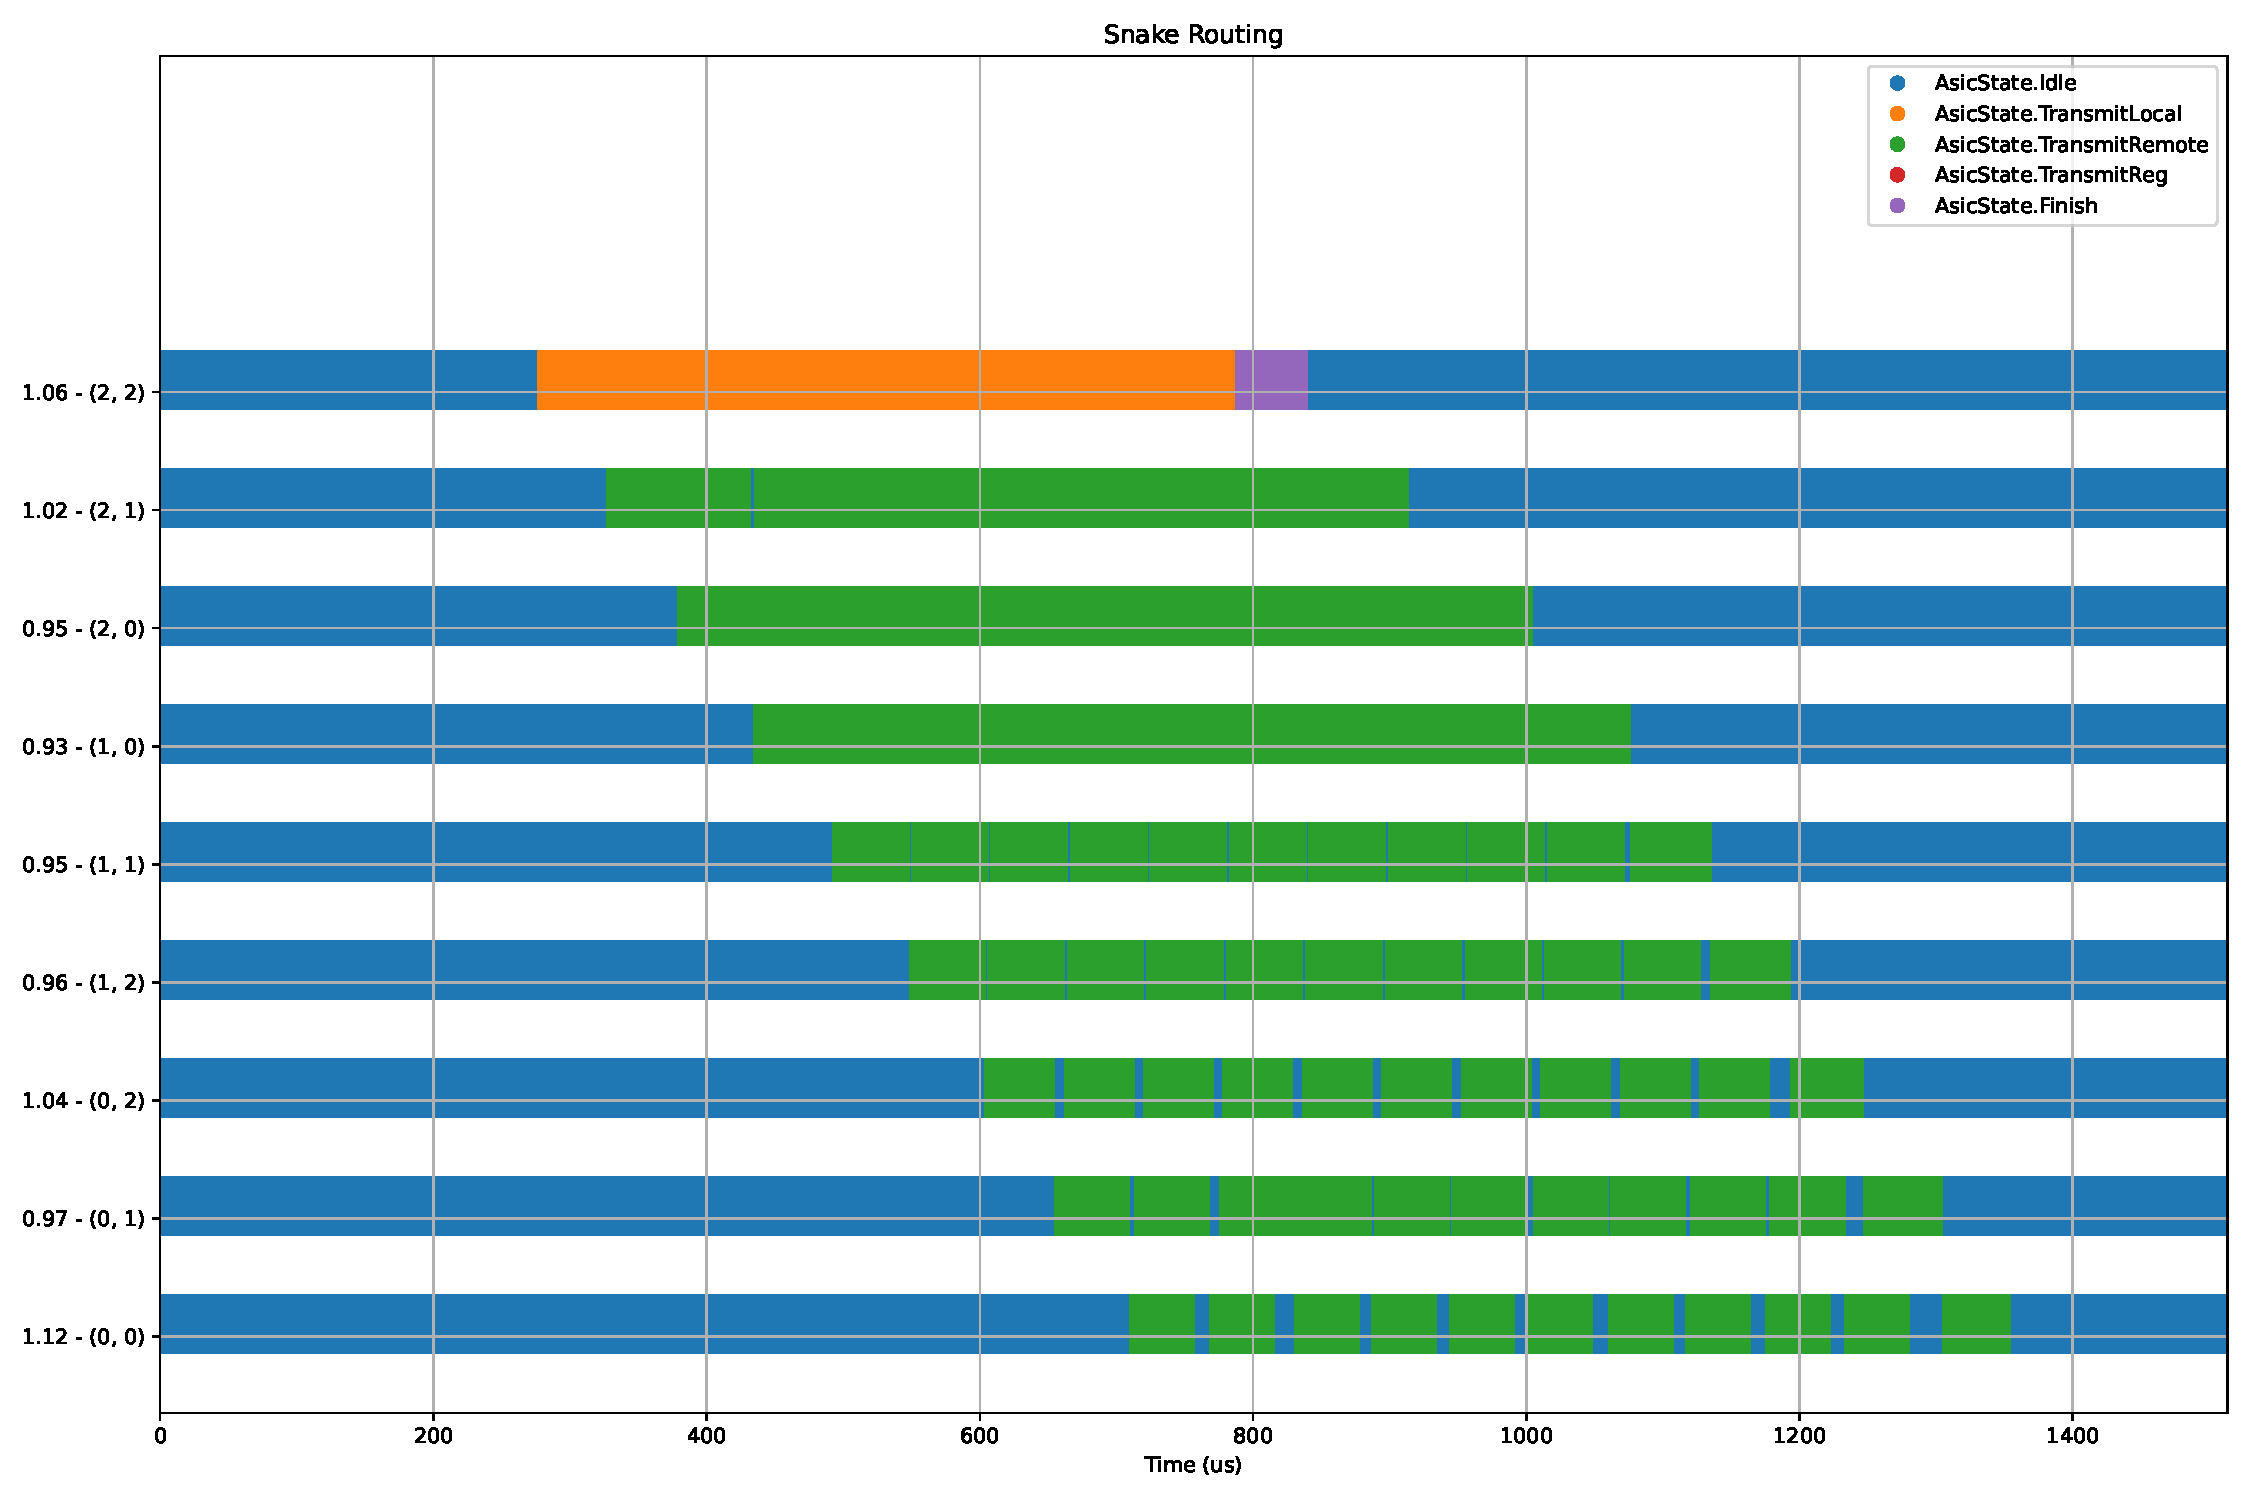
\includegraphics[width=\textwidth]{images/snake_timer.pdf}
  \caption{Snake Readout timing Diagram}
\end{subfigure}%
\begin{subfigure}{.5\textwidth}
  \centering
  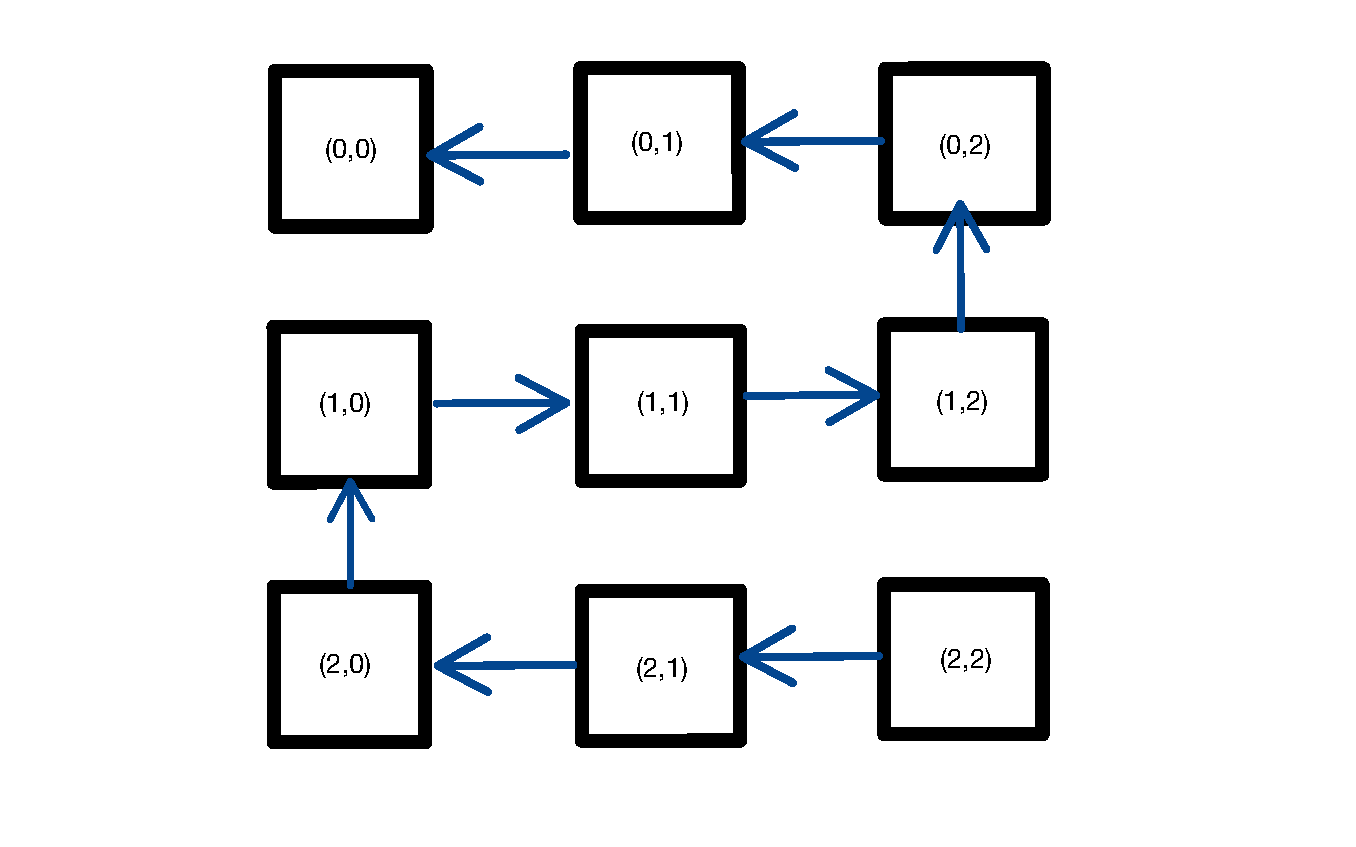
\includegraphics[width=\textwidth]{images/snake_ex_read.pdf}
  \caption{Data Path in Snake Readout}
\end{subfigure}
\caption{Snake Packet Transaction Example}
\label{fig:snake_packet_drift}
\end{figure}


\begin{figure}
\centering
\begin{subfigure}{.5\textwidth}
  \centering
  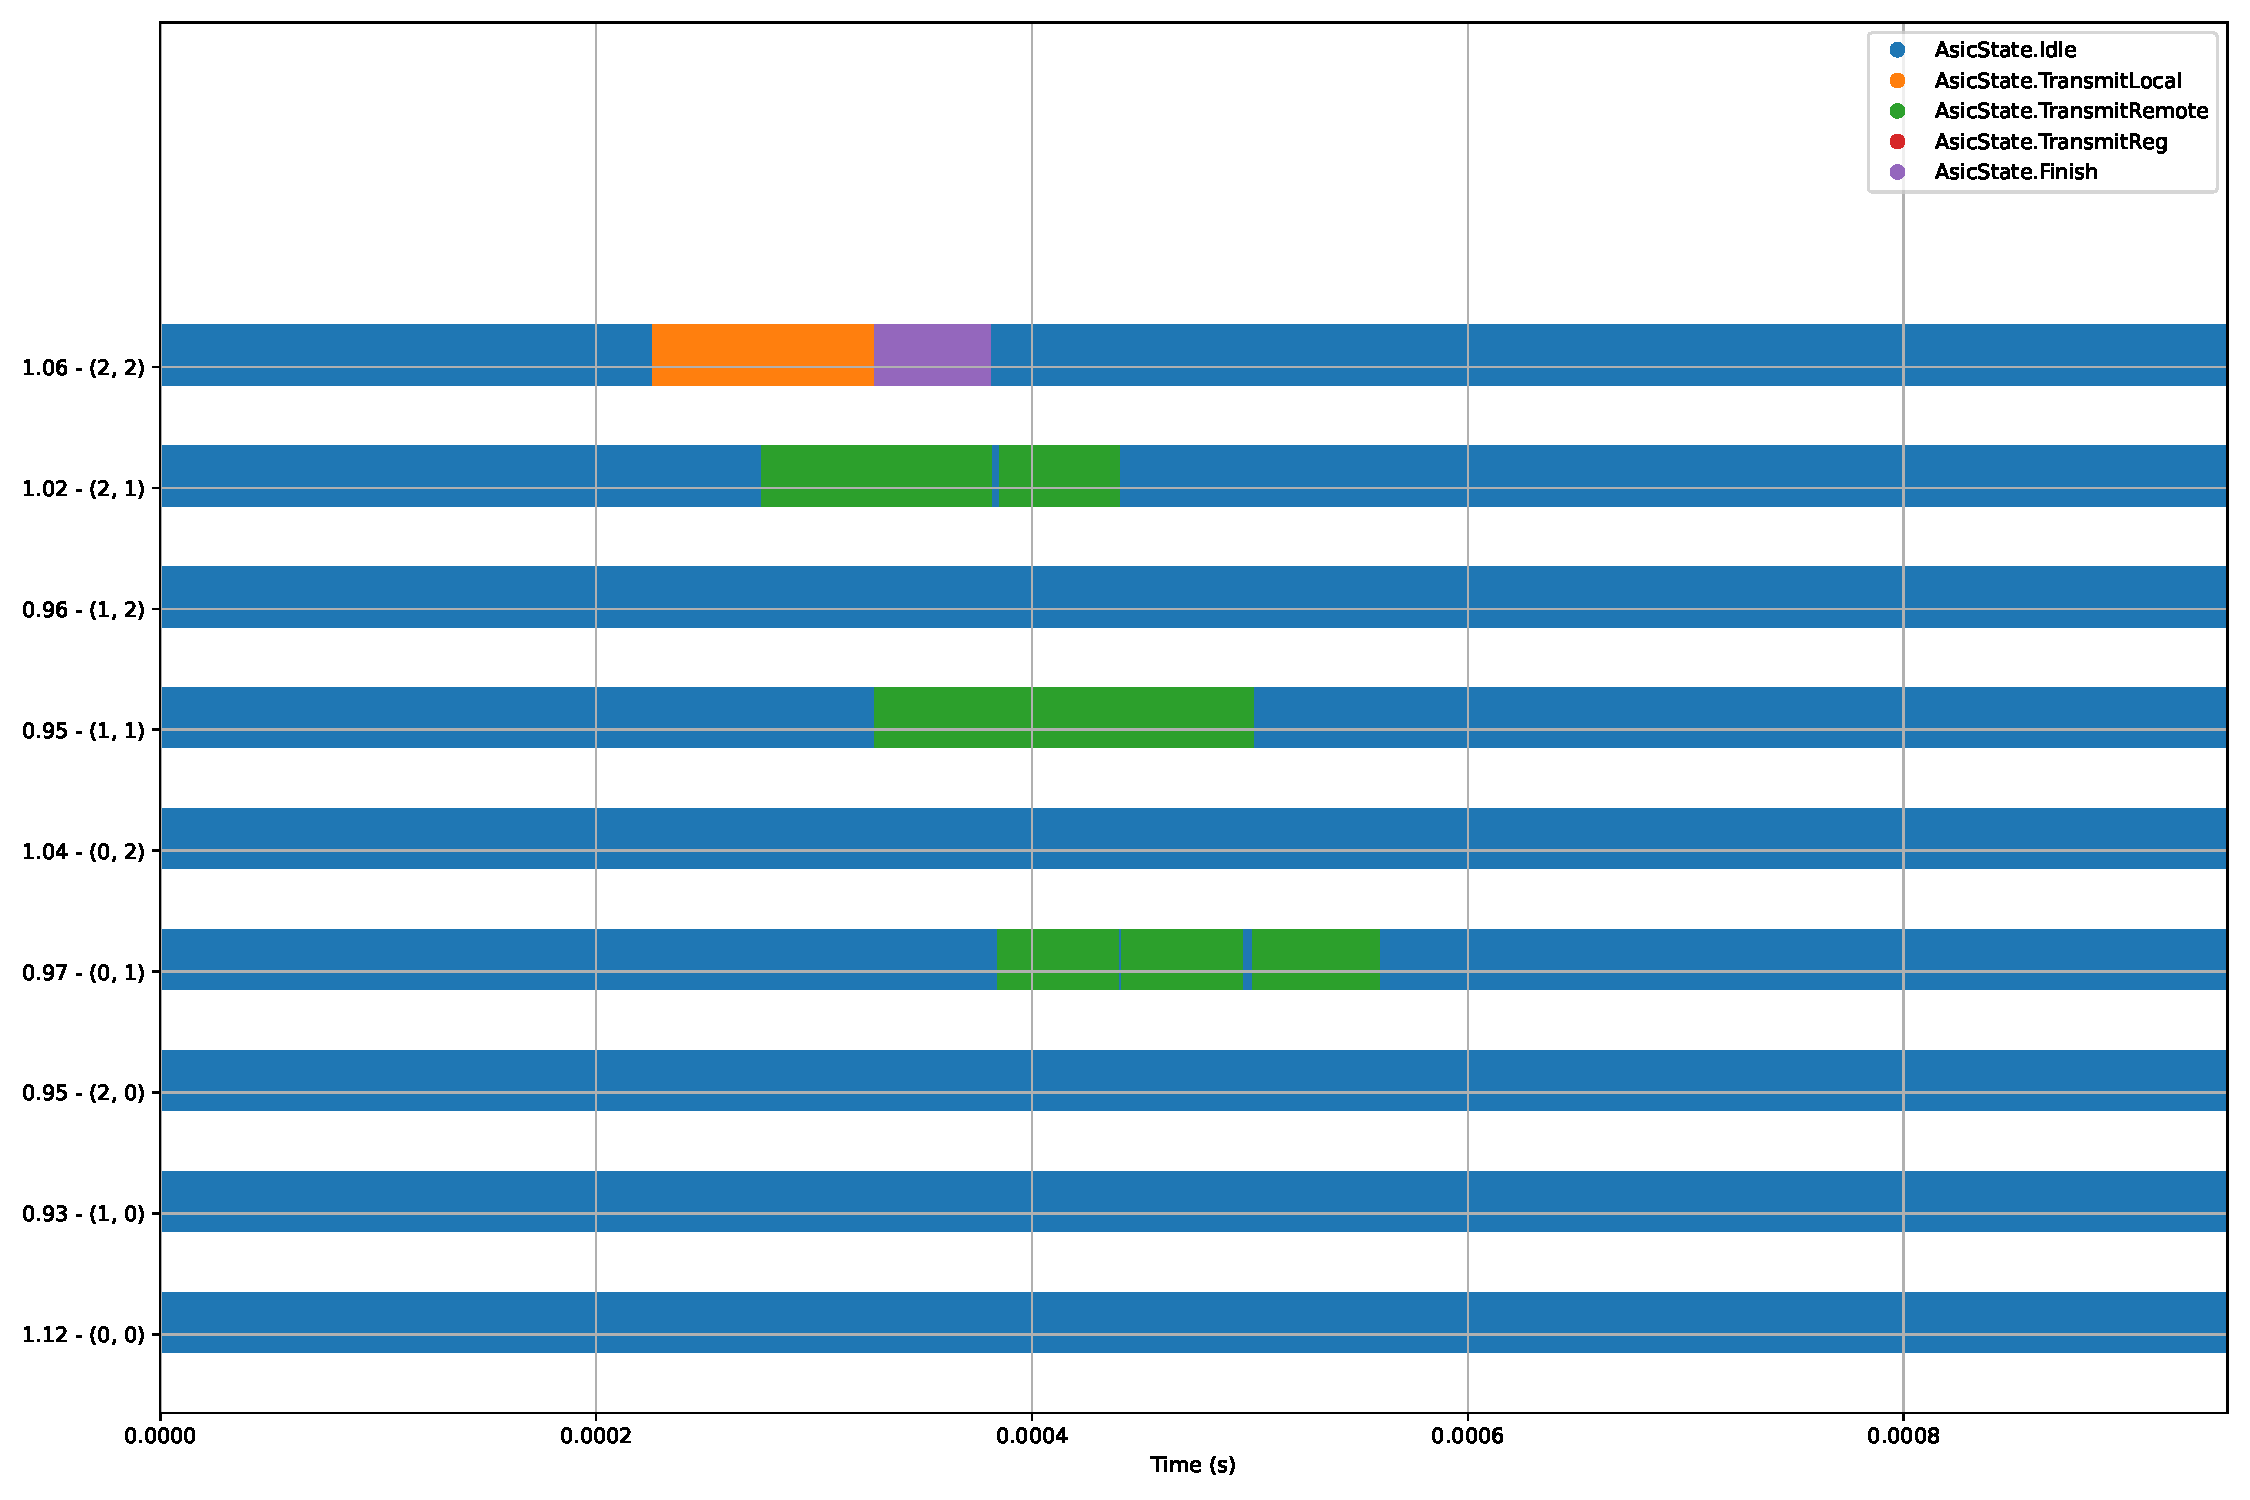
\includegraphics[width=\textwidth]{images/trunk_timer.pdf}
  \caption{Trunk Readout timing Diagram}
\end{subfigure}%
\begin{subfigure}{.5\textwidth}
  \centering
  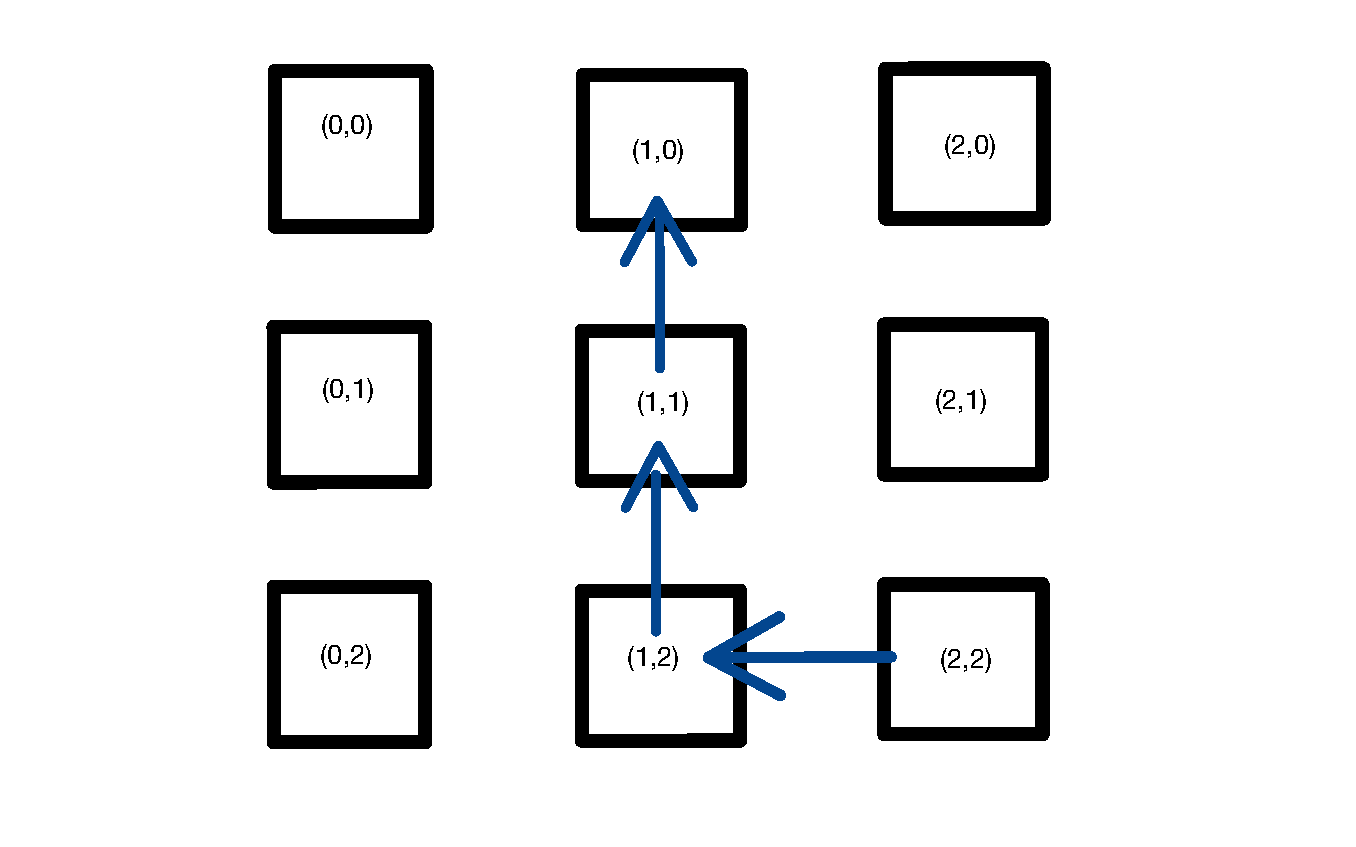
\includegraphics[width=\textwidth]{images/trunk_ex_read.pdf}
  \caption{Data Path in Trunk Readout}
\end{subfigure}
\caption{Trunk Packet Transaction Example}
\label{fig:trunk_packet_drift}
\end{figure}


\begin{figure}
\centering
\begin{subfigure}{.5\textwidth}
  \centering
  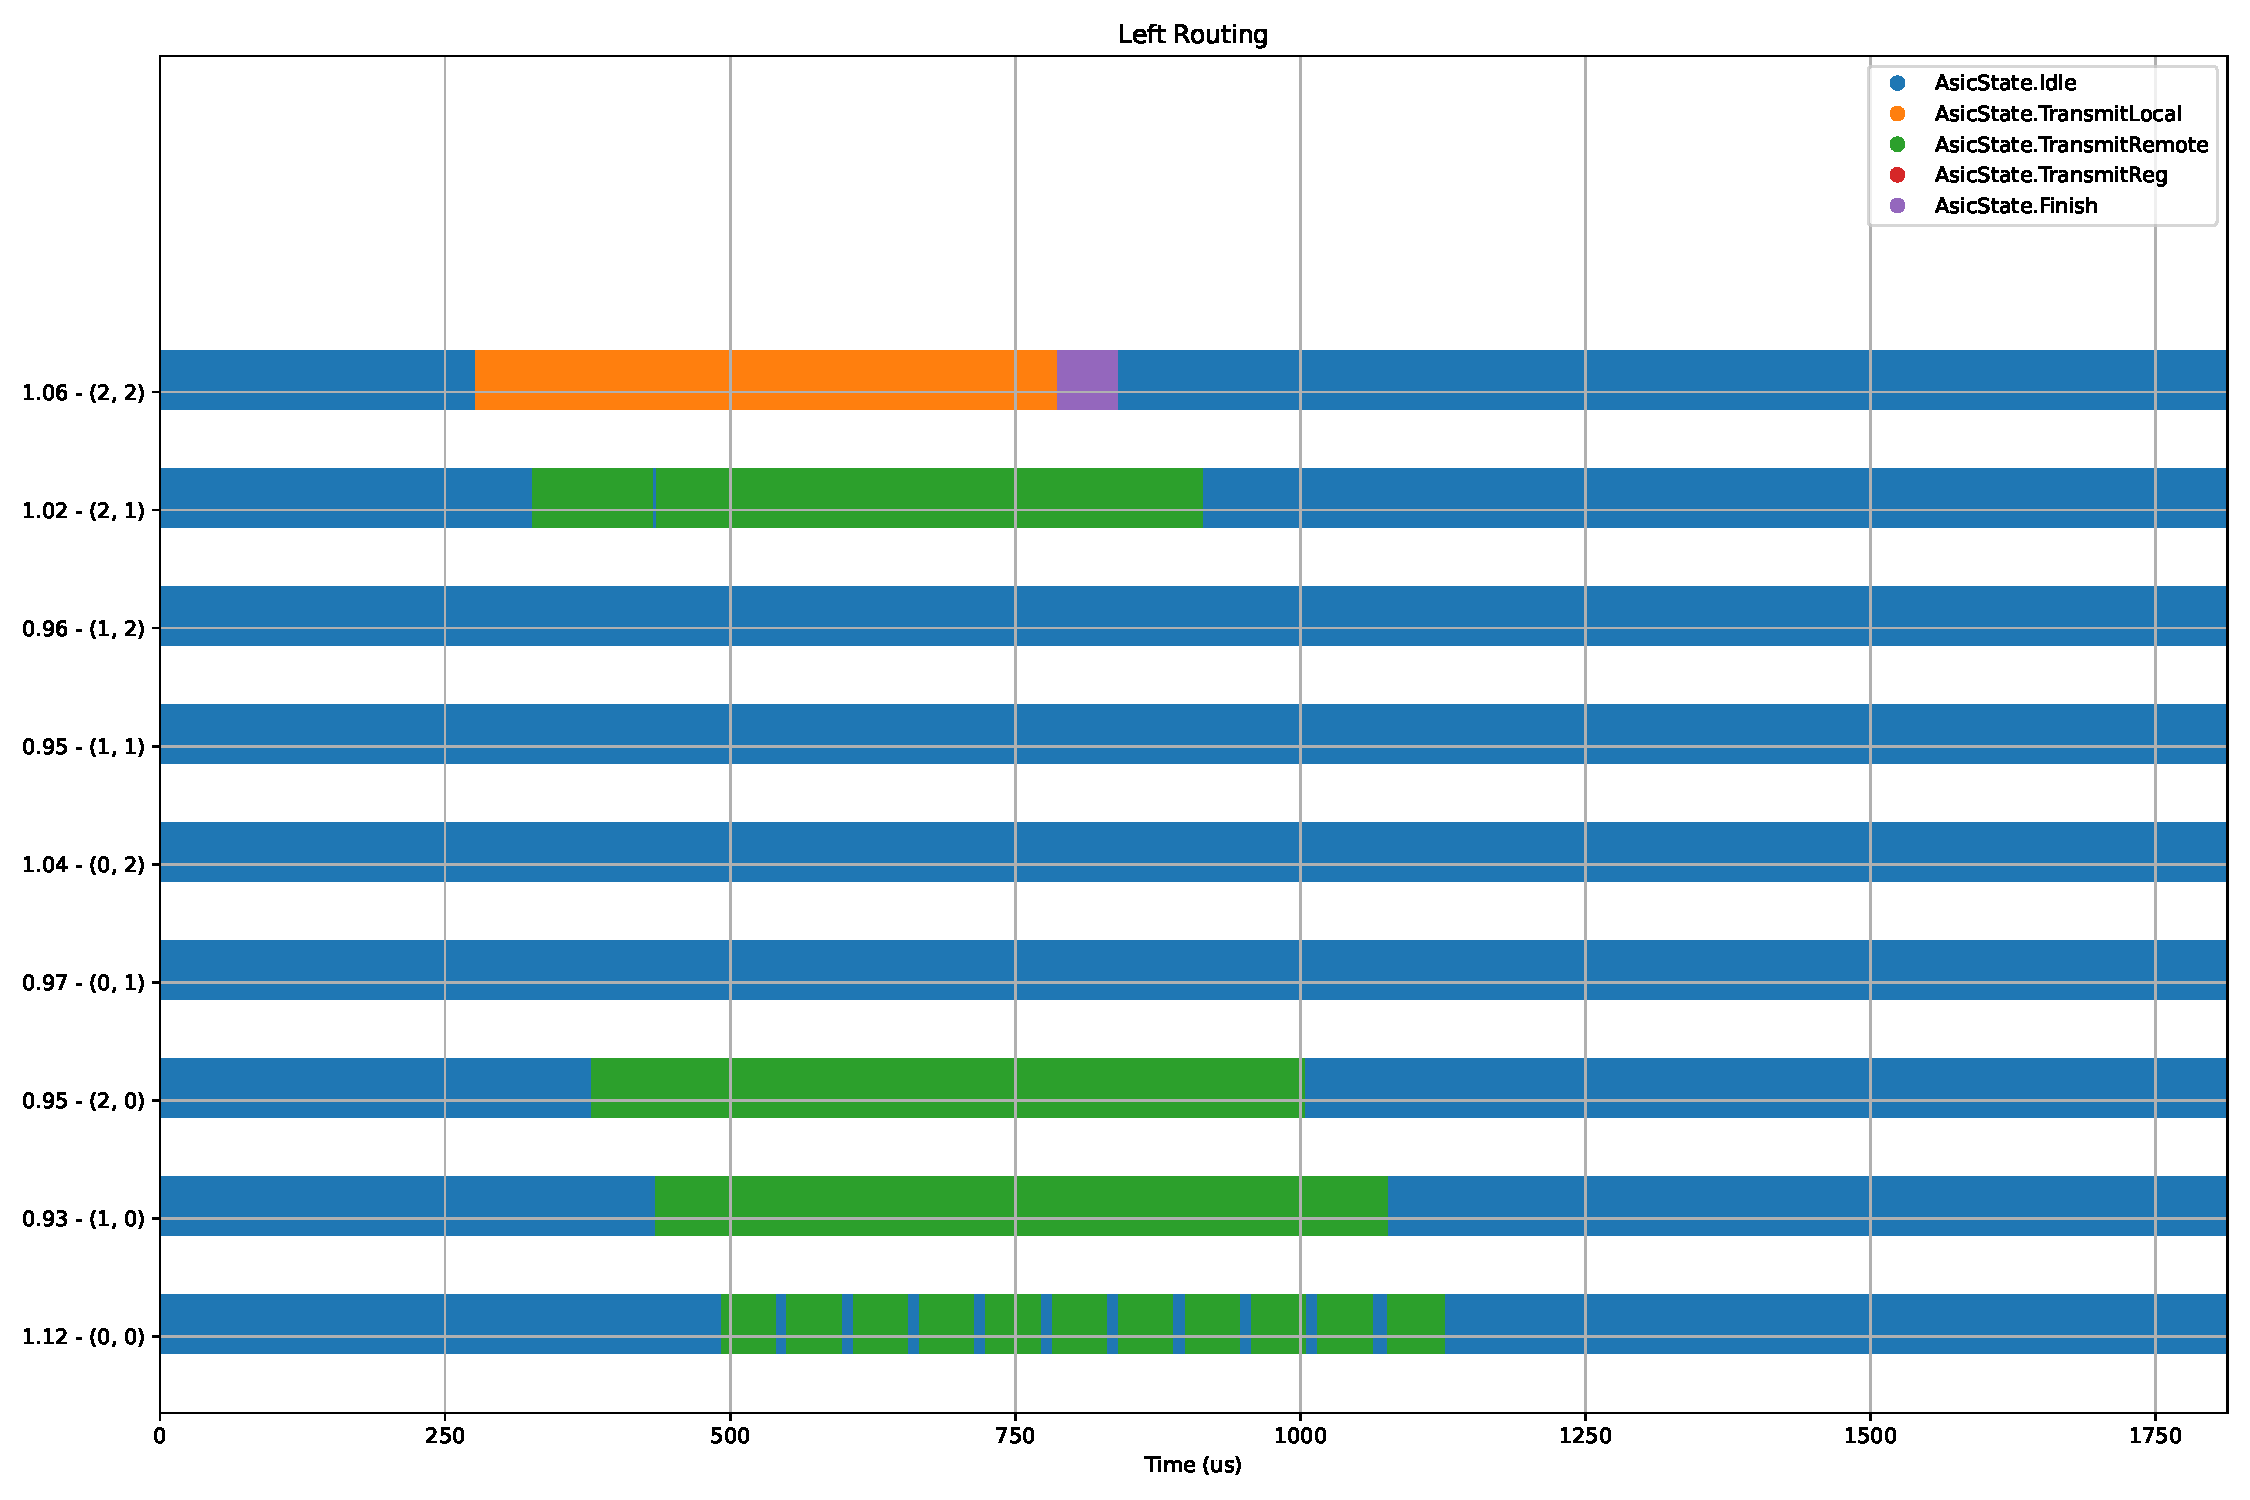
\includegraphics[width=\textwidth]{images/left_timer.pdf}
  \caption{Left Readout timing Diagram}
\end{subfigure}%
\begin{subfigure}{.5\textwidth}
  \centering
  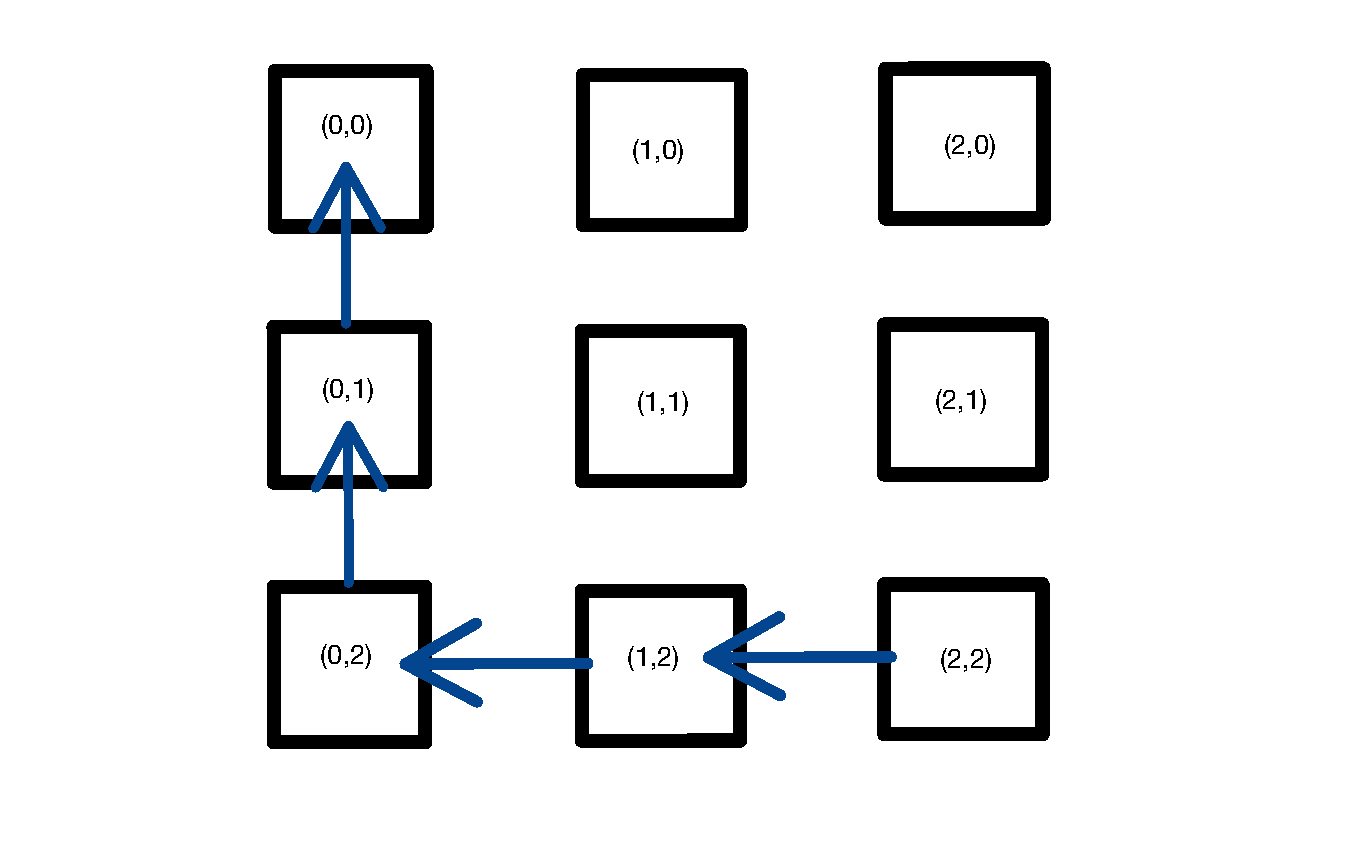
\includegraphics[width=\textwidth]{images/left_ex_read.pdf}
  \caption{Data Path in Left Readout}
\end{subfigure}
\caption{left Packet Transaction Example}
\label{fig:left_packet_drift}
\end{figure}

%% example local vs remote of left
\begin{figure}
\centering
\begin{subfigure}{.5\textwidth}
  \centering
  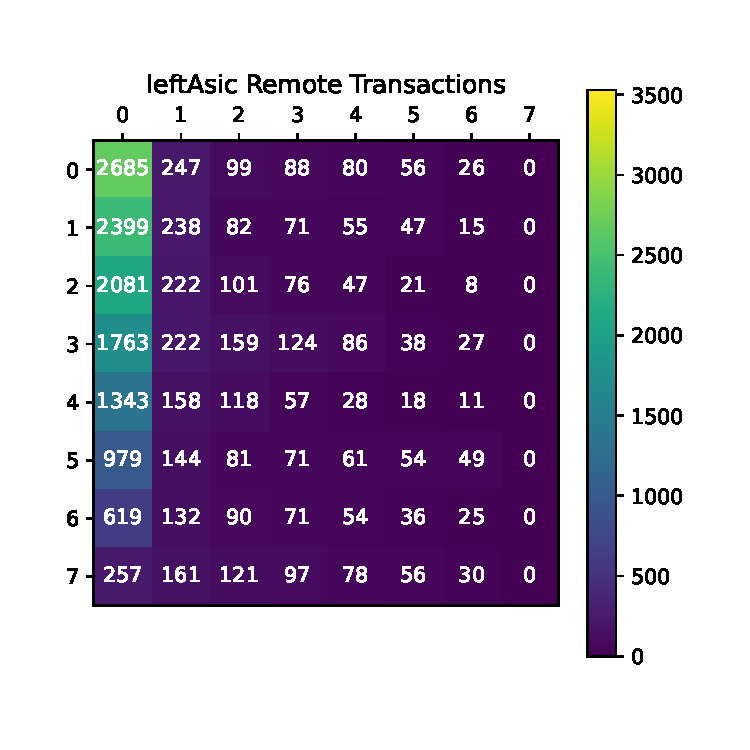
\includegraphics[width=\textwidth]{images/left_asic_trans.pdf}
  \caption{Local FIFO Depths}
\end{subfigure}%
\begin{subfigure}{.5\textwidth}
  \centering
  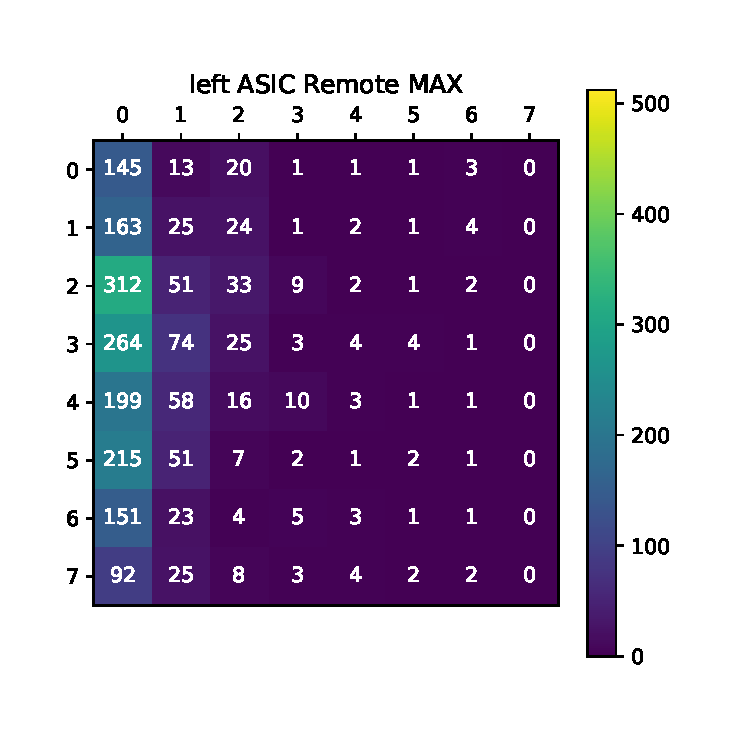
\includegraphics[width=\textwidth]{images/left_asic_remote.pdf}
  \caption{Remote FIFO Depths}
\end{subfigure}
\caption{Example of local (a) and Remote (b) fifo depths of the example neutrino event after processing.}
\label{fig:left_example_neutrino}
\end{figure}

%% example local vs remote of trunk
\begin{figure}
\centering
\begin{subfigure}{.5\textwidth}
  \centering
  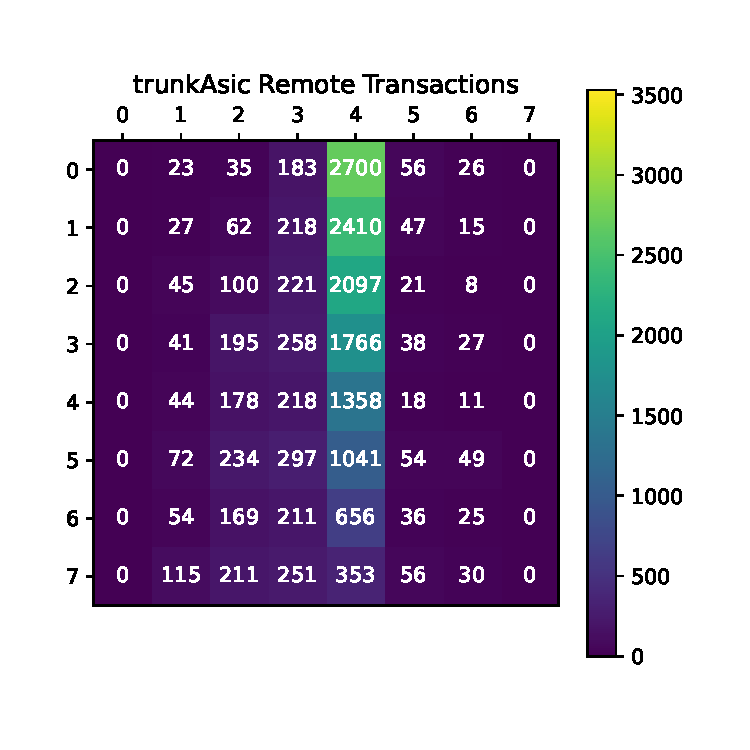
\includegraphics[width=\textwidth]{images/trunk_asic_trans.pdf}
  \caption{Local FIFO Depths}
\end{subfigure}%
\begin{subfigure}{.5\textwidth}
  \centering
  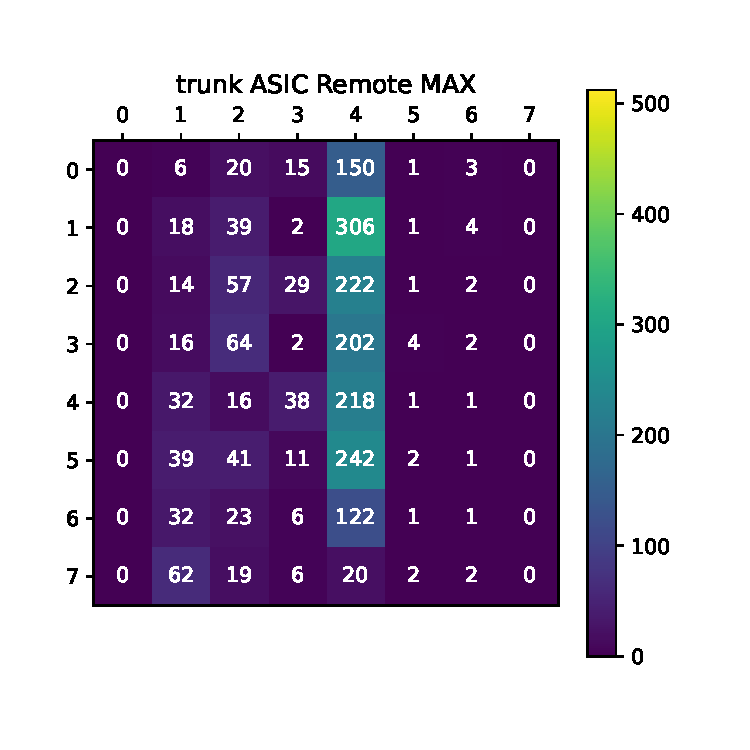
\includegraphics[width=\textwidth]{images/trunk_asic_remote.pdf}
  \caption{Remote FIFO Depths}
\end{subfigure}
\caption{Example of local (a) and Remote (b) fifo depths of the example neutrino event after processing.}
\label{fig:trunk_example_neutrino}
\end{figure}

\subsection{The Push Architecture}

\begin{figure}[]
\centering
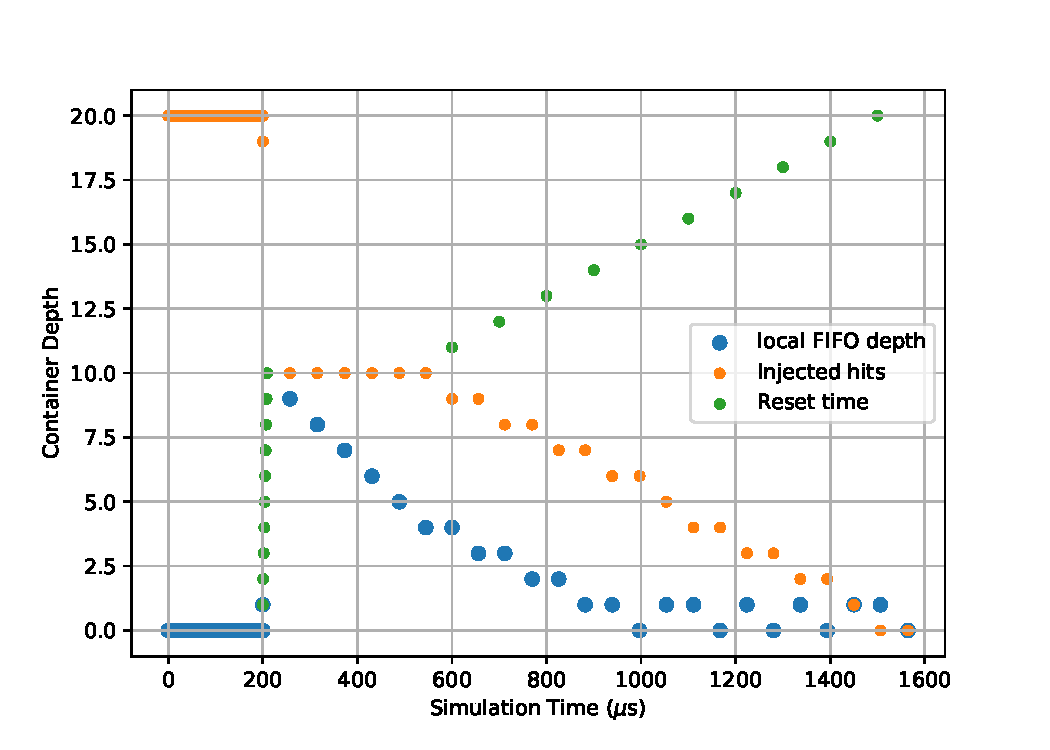
\includegraphics[width=\textwidth]{images/push_arch_buff.pdf}
\caption{A simulated push Architecture with injected hits.}
\end{figure}~\label{fig:push_arch_verification}
